%%%%%%%%%%%%%%%%%%%%%%%%%%%%%%%%%%%%%%%%%%%%%%%%%%%%%%%%%%%%%%%%%%%%
%% I, the copyright holder of this work, release this work into the
%% public domain. This applies worldwide. In some countries this may
%% not be legally possible; if so: I grant anyone the right to use
%% this work for any purpose, without any conditions, unless such
%% conditions are required by law.
%%%%%%%%%%%%%%%%%%%%%%%%%%%%%%%%%%%%%%%%%%%%%%%%%%%%%%%%%%%%%%%%%%%%

\documentclass{beamer}
\usetheme[logopath=./, logo=fig/logo-tu.png]{fibeamer}
\usepackage[utf8]{inputenc}
\usepackage[
  main=english, %% By using `czech` or `slovak` as the main locale
                %% instead of `english`, you can typeset the
                %% presentation in either Czech or Slovak,
                %% respectively.
  czech, slovak %% The additional keys allow foreign texts to be
]{babel}        %% typeset as follows:
%%
%%   \begin{otherlanguage}{czech}   ... \end{otherlanguage}
%%   \begin{otherlanguage}{slovak}  ... \end{otherlanguage}
%%
%% These macros specify information about the presentation
\title{Detecting Empty Frame Objects On MAVs Using Synthetic Data} %% that will be typeset on the
\subtitle{Applied in Autonomous Drone Racing} %% title page.
\author{Philipp Dürnay\\ \bigskip \bigskip Prof. Guido de Croon \hfill	
\includegraphics[width=3cm]{fig/mavlab}\\
	 Prof. David M. J. Tax  \hfill 
\includegraphics[width=3cm]{fig/prgroup}%
}
%% These additional packages are used within the document:
\usepackage{ragged2e}  % `\justifying` text
\usepackage{booktabs}  % Tables
\usepackage{tabularx}
\usepackage{tikz}      % Diagrams
\usetikzlibrary{calc, shapes, backgrounds}
\usepackage{amsmath, amssymb}
\usepackage{url}       % `\url`s
\usepackage{listings}  % Code listings
\frenchspacing
\begin{document}
  \frame{\maketitle}

  %\AtBeginSection[2,3,4]{% Print an outline at the beginning of sections
  %  \begin{frame}<beamer>
  %    \frametitle{Outline for Section \thesection}
  %    \tableofcontents[currentsection]
  %  \end{frame}}

  \begin{darkframes}
  	\begin{frame}{Outline}
  		\tableofcontents
  	\end{frame}
	\section{Introduction}
%	\subsection{Application}
    \begin{frame}{Application}
    	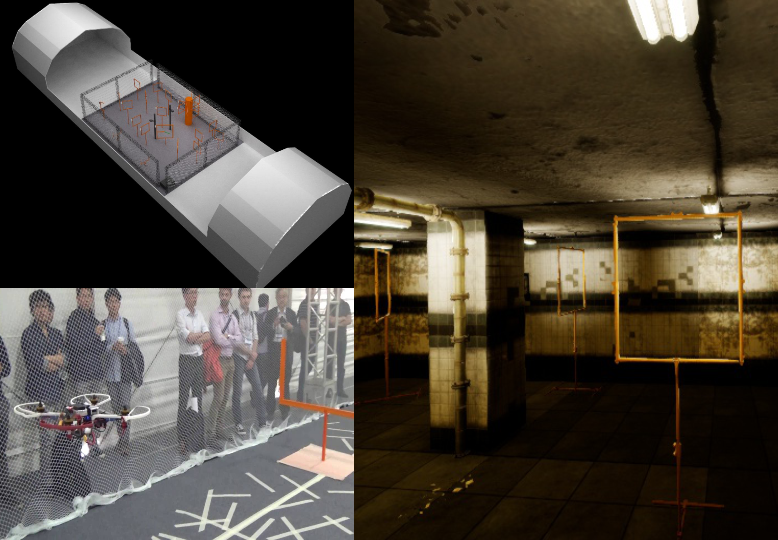
\includegraphics[width=\textwidth]{fig/application}
    \end{frame}
%So we start with the background. The final application will be at the Autonomous Drone Race at the IROS2018 conference in spain. There you have a track that consists of multiple orange gates that need to be passed one after another. So here on the top you see the race court of two years ago. On the bottom you see an example of how a drone looks like. And here on the right you see an example of the training data. So in our method we use these gates to determine our own position. So we detect the gate estimate our own position relative to it and then this goes to the control loop and we fly through. In my thesis I am concerned with the detection of these gates.

%Now currently we have a very basic computer vision method that basically looks for orange pixels and if it finds a square it extracts the corners and together with the known geometry of the gate we can estimate our own position.
%As you can imagine this method is purely colour based and very brittle. You need to tune the colour values depending on the light conditions of the room. And even then if you have strong shadows the method fails. Also it can happend that you are quite far away from the gate and then you don't see the square anymore but only the pole. In this case the method also doesnt work. So we want to improve this by using a learning based approach. As we hope this results in a more robust and flexible method. For example a learning based method you can train if the shapes of the gate change. So this brings me to the underlying research problem. Which can be formulated as follows.

\begin{frame}{Pipeline}
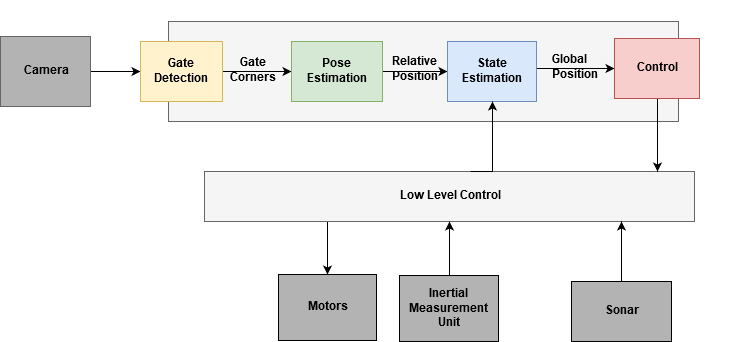
\includegraphics[width=\textwidth]{fig/control_loop_inv}
\end{frame}
%\subsection{Challenges}    
\begin{frame}
\centering
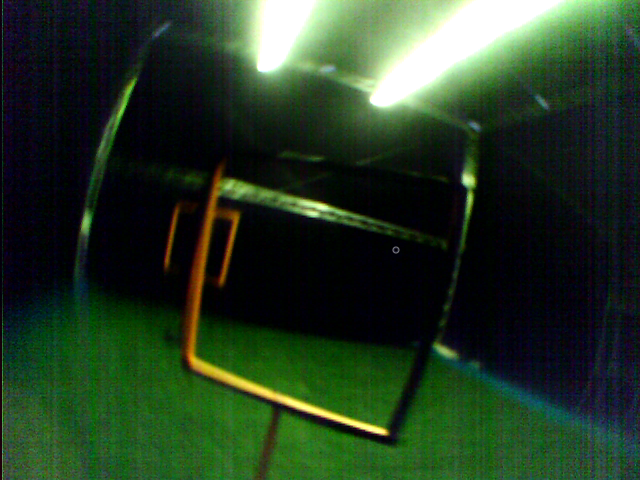
\includegraphics[width=0.31\textwidth]{../../thesis/fig/real_cyberzoo1.png}
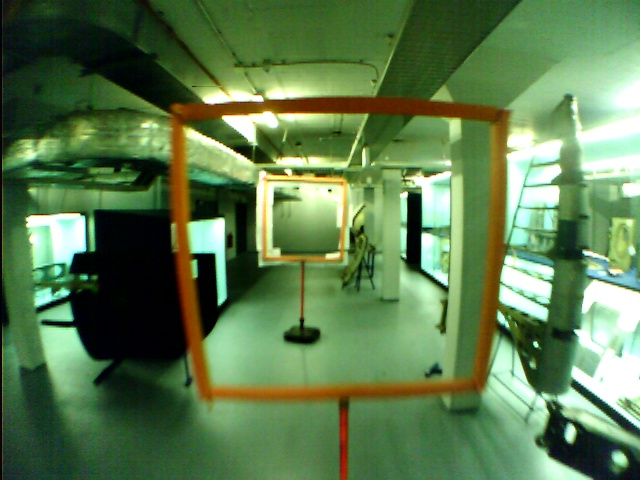
\includegraphics[width=0.31\textwidth]{../../thesis/fig/basement}
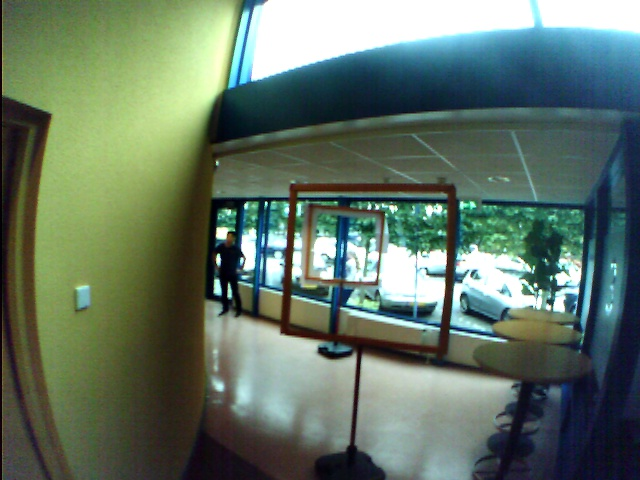
\includegraphics[width=0.31\textwidth]{../../thesis/fig/hallway}
\begin{block}{Challenges}
	\begin{enumerate}
		\item Objects consist of thin structures that are spread over large parts of the image.
		
		\item Fast motion, lens distortion and illumination affect object appearance.
		
		\item On board resources are limited.
		
		\item Limited annotated examples are available.
		
	\end{enumerate}
\end{block}
\end{frame}

%	\subsection{Research Question}    
	\begin{frame}	
	\textbf{How can we use synthetic data to learn an object detector for empty wireframe objects on a micro-air vehicle?\\}
	\bigskip

	\centering
   	%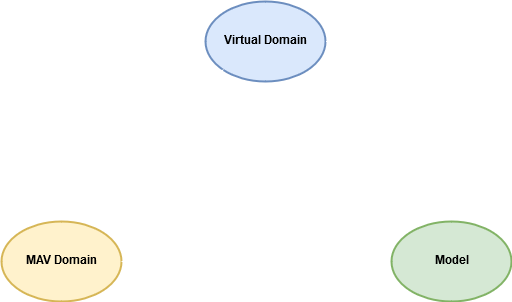
\includegraphics[width=0.8\textwidth]{fig/triangle_white}
	\end{frame}
%\begin{frame}	
%\textbf{How can we use synthetic data to learn an object detector for empty wireframe objects %on a micro-air vehicle?\\}
%\bigskip

%\centering
%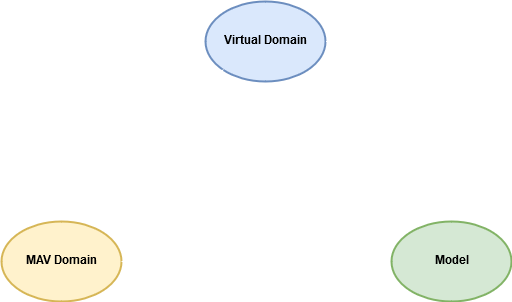
\includegraphics[width=0.8\textwidth]{fig/triangle_white}
%\end{frame}
 % Since it needs to run on a drone it should be fast and the faster it gets the better for the control, the faster we can fly/ a smaller drone we can use. The wire frame objects we refer to as the objects we want to detect consists only out of a thin frame but I will get back to that later. So I will look at some background in object detection.   
    \section{Background}
    \begin{frame}{Outline for Section \thesection}
    \tableofcontents[currentsection]
	\end{frame}
%\subsection{Object Detection}
	\begin{frame}{Object Detection}
	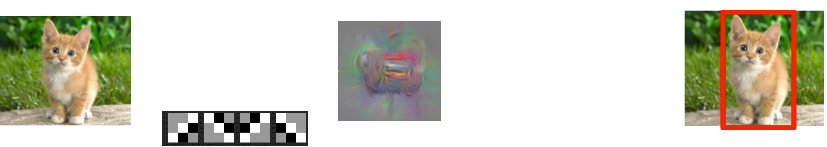
\includegraphics[width=\textwidth]{fig/ObjectDetection}
	\end{frame}
% if you look at object detection on a high level basis, you basically see this pipeline
% You have your input image and at the end you want to have a bounding box that tells you which object is where in the image for example with such a bounding box,
% so usually you preprocess the image by extracting certain features from the image
% so you have filters that look for certain colours or an eye or an ear for example,
% this gives you an internal representation of the image with the important aspects
% then you do two tasks and that is classification and localization so determining the object and the bounding box coordinates
% Now there are different ways for each of these steps but thats it from a high level perspective
% State of the art methods all use convolutional neural networks and the reason that is beliefed to be responsible for that performance is the fact that you can combine all these steps in one model and train it end to end on the task so instead of manually enginnering and training models you combine it all in one.
%	\subsection{Convolutional Neural Networks}
		\begin{frame}{Convolutional Neural Networks}
	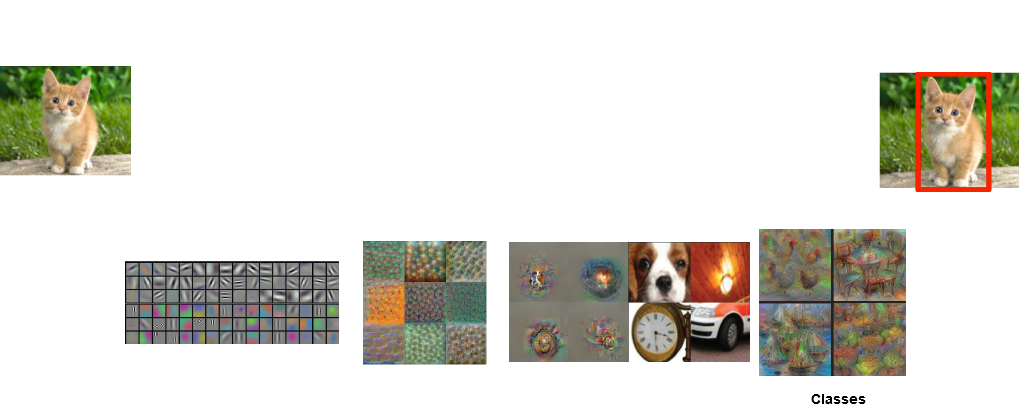
\includegraphics[width=\textwidth]{fig/cnn_mine}
\end{frame}

%\begin{frame}{One Stage Detectors}
%$$
%\mathcal{L} = \sum_{i=0}^{S^2}\sum_{j=0}^B\mathbf{1}_{ij}^{obj}(\lambda_{loc}\mathcal{L}_{loc} %+ \lambda_{obj}\mathcal{L}_{obj} + \lambda_{class}\mathcal{L}_{class}) + %\mathbf{1}_{ij}^{noobj}(\lambda_{noobj}\mathcal{L}_{noobj})
%$$
%
%\end{frame}
\section{Hypothesis}
\begin{frame}{Hypothesis}
    \begin{itemize}
    	\item A deep network can learn more robust features
    	\item A simple network should be able to learn the task
    	\item Simulating the real world can improve the performance in the real world
    \end{itemize}
\end{frame}
% So now we can look at an example for a convolutional network and at the different layers. So typically you apply per layer a certain amount of filters, then you apply pooling and non-linearity and you stack several of these filters and at the end you have your output.
% And typically the performance improves the deeper you go. One reason is that the flexibility of the model increases but you can also look at it from another perspective and see what the different layers are responsible for. So when you visualize these filters you usually see how these early layers look for edges, corner and blobs, while higher layers then combine these low level features to more complex parts like eyes, noses and so on.
% Now the draw back of these deep networks is their computational effort, especially the deep one is their huge consumption in energy, computations and memory which makes them not applicable for micro air vehicles.
% But if we now rethink to the objects we want to detect so wire frame objects, racing gates that mostly consist of edges and corners, these final layers should not be very useful. So a much smaller model should actually be sufficient. 
    \section{Experiments}
        \begin{frame}{Outline for Section \thesection}
    \tableofcontents[currentsection]
\end{frame}

\begin{frame}{Experimental Setup}
\centering
\begin{itemize}
	\item Synthetic Trainingset 20 000 samples
	\item Synthetic Testset 550 samples, 1361 objects
	\item Real Dataset 300 samples, 423 objects
	\item Metric: Average Precision
\end{itemize}
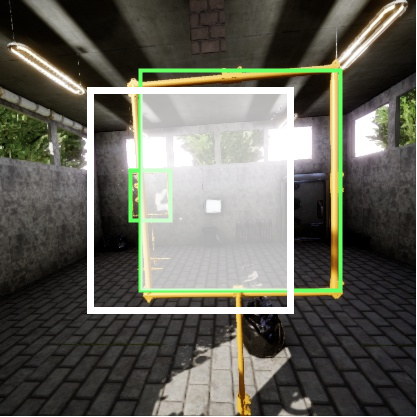
\includegraphics[width=0.3\textwidth]{fig/iou_example}

\end{frame}

\begin{frame}{Synthetic Data}
\centering
\includegraphics[width=0.45\textwidth]{../../thesis/fig/daylight_perspective}
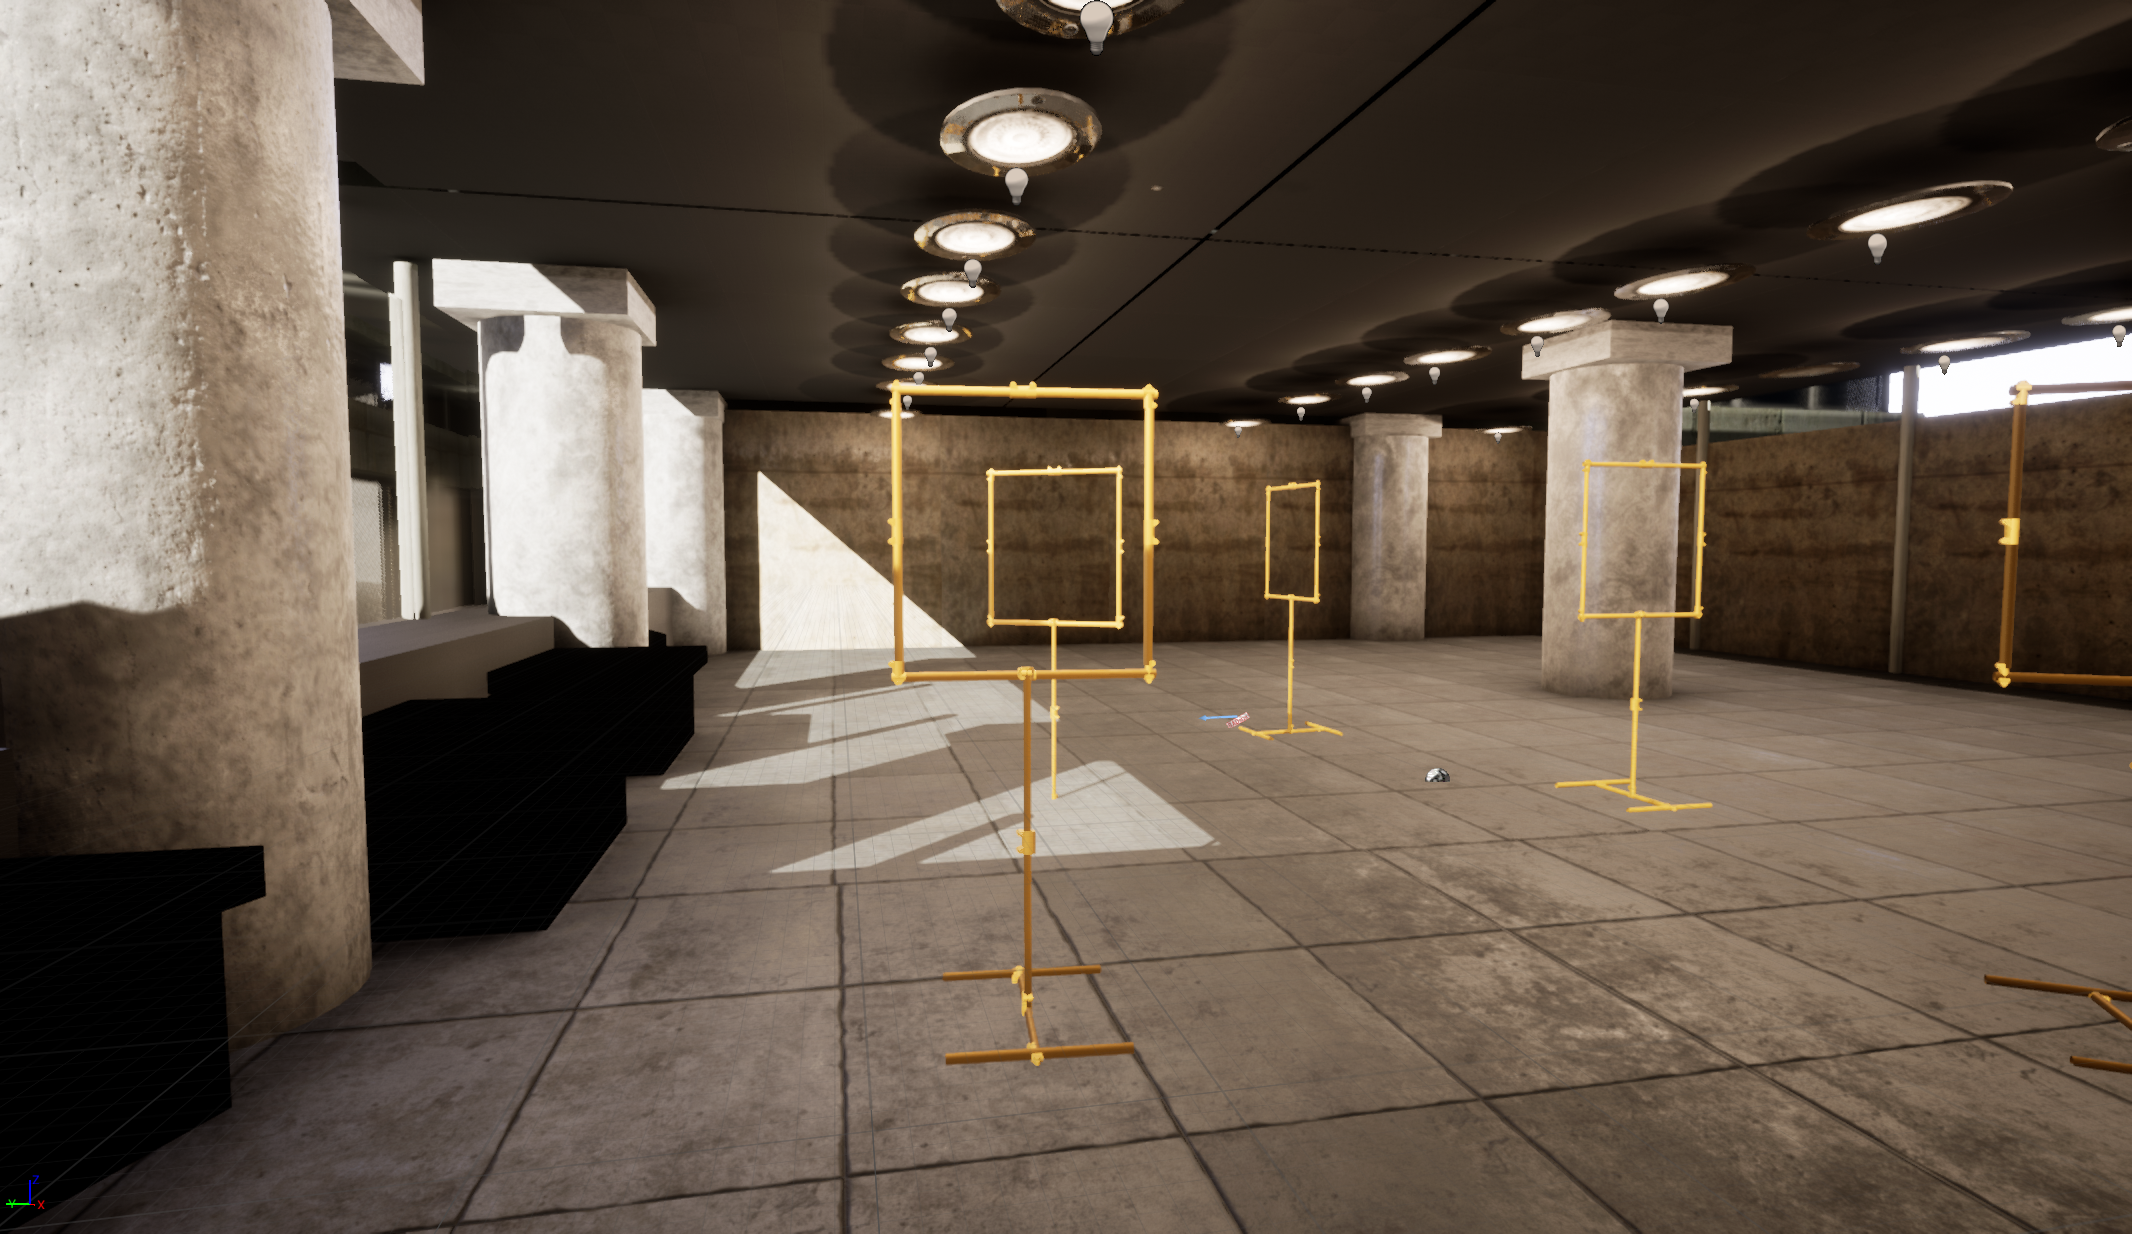
\includegraphics[width=0.45\textwidth]{../../thesis/fig/iros_perspective}
\end{frame}

\begin{frame}{Real Dataset}
\centering
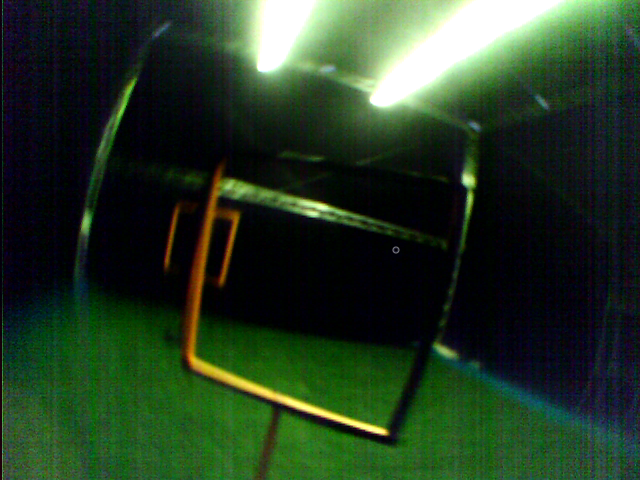
\includegraphics[width=0.31\textwidth]{../../thesis/fig/real_cyberzoo1.png}
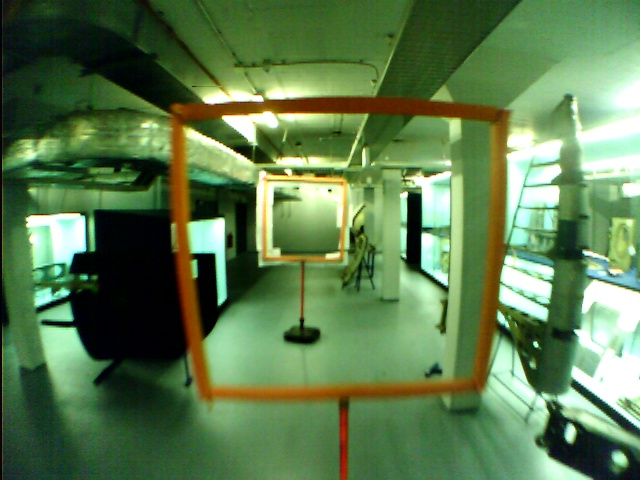
\includegraphics[width=0.31\textwidth]{../../thesis/fig/basement}
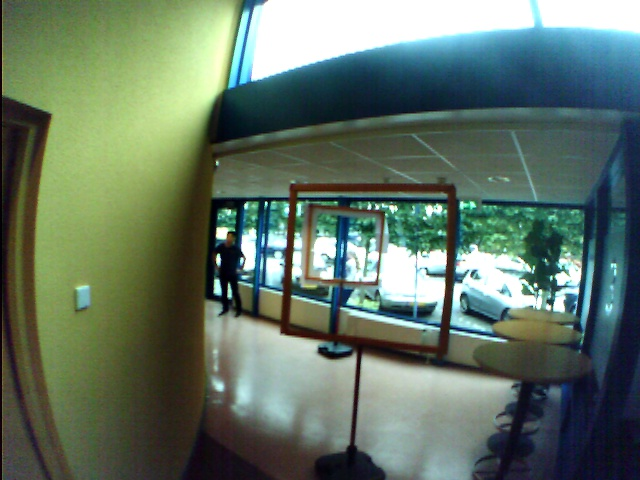
\includegraphics[width=0.31\textwidth]{../../thesis/fig/hallway}
\end{frame}

%\subsection{Network Design}

\begin{frame}{Results}
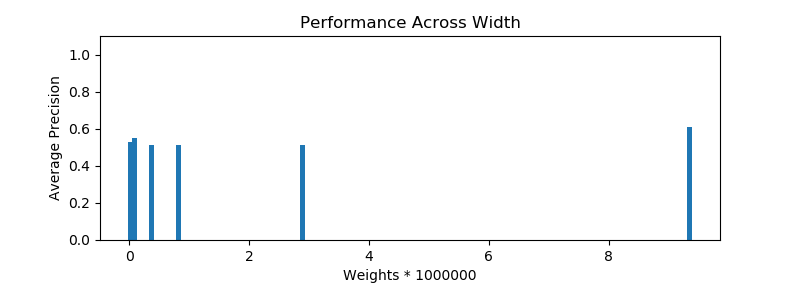
\includegraphics[width=\textwidth]{../../thesis/fig/perf_width}
\end{frame}

\begin{frame}{Results}
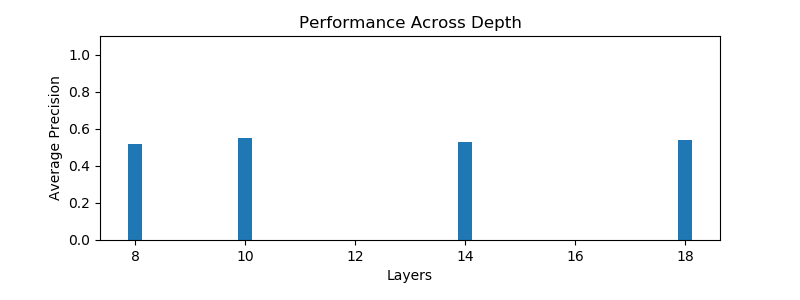
\includegraphics[width=\textwidth]{../../thesis/fig/perf_depth}
\end{frame}
 % \subsection{Data Generation}
%    \begin{frame}{Data Properties}
%\begin{itemize}
%	\item \textbf{Background/Environment} \\Illumination, Background Texture, Other Objects
%	\item \textbf{View} \\Appearance of the object relative to the camera
%	\item \textbf{Sensor Effects} \\Motion Blur, Chromatic/Geometric Distortion
%\end{itemize}
%    \end{frame}


    \begin{frame}{Sensor Effects}
\begin{itemize}
	\item Motion Blur 
	\item Chromatic Aberration
	\item Exposure
	\item HSV variations
\end{itemize}
\end{frame}
    \begin{frame}{Sensor Effects}
    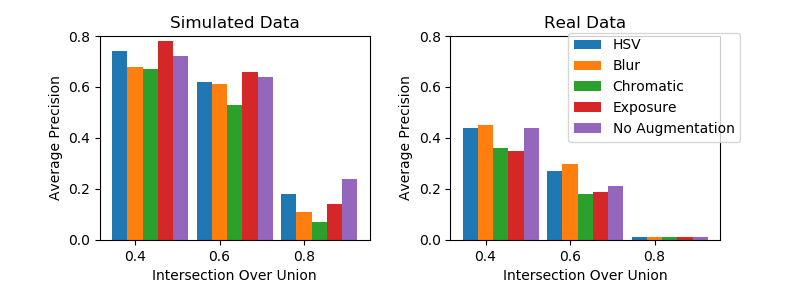
\includegraphics[width=\textwidth]{../../thesis/fig/pp_bar}
	\end{frame}


%  \subsection{Comparison to Baseline}
      \begin{frame}{Comparison to Baseline}
      \centering
    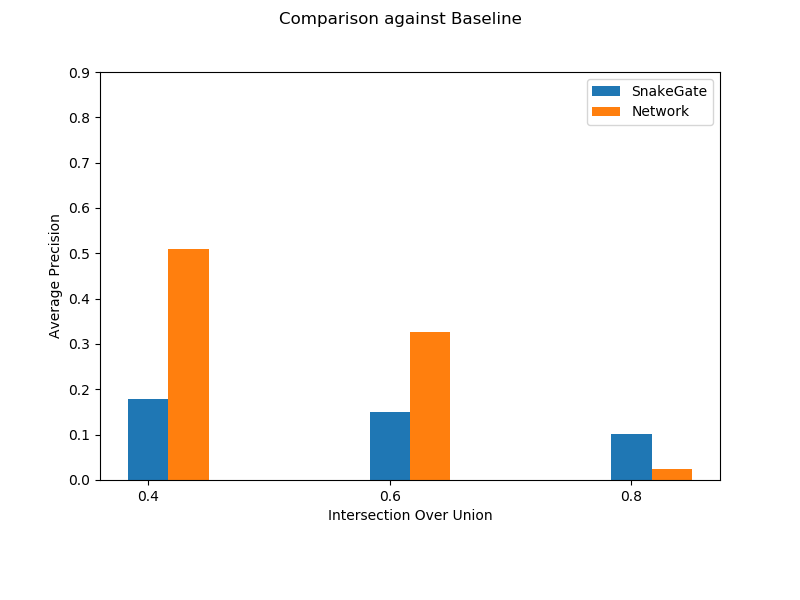
\includegraphics[width=0.8\textwidth]{../../thesis/fig/comp_baseline}
	\end{frame}

    
    \section{Conclusion}
 %      \subsection{Conclusion}
            \begin{frame}{Outline for Section \thesection}
    \tableofcontents[currentsection]
\end{frame}
    \begin{frame}{Conclusion}

    \begin{itemize}
    	\item Small Network is able to learn the task equally well than bigger network
    	\item Image Augmentation by applying image blur and variations in HSV improve the localization on the real data
    	\item Chromatic Aberration and variations in Exposure have small influence or lead to a deterioration in performance
    	\item Network performs better than baseline but bounding boxes are less accurate
    	\item Trade-Off in speed/accuracy
    \end{itemize}
    \end{frame}

 %  \subsection{Open Questions}
       \begin{frame}{Open Questions}
\begin{itemize}
	\item Reality Gap
	\item Localization Error high
  \end{itemize} 
\end{frame}
    \begin{frame}{Questions}
    \centering
\huge ?
    	\end{frame}
    
    
  \end{darkframes}

\end{document}
